\documentclass[12pt]{article}  

\usepackage[boxruled,lined]{algorithm2e}
%% \usepackage{booktabs}
\usepackage{amsmath} 
\usepackage{amsthm} 
\usepackage{amsfonts} 
\usepackage{enumitem}
\usepackage[T1]{fontenc}
\usepackage[utf8]{inputenc}
\usepackage{xparse} 
\usepackage{bm}
\usepackage{bbm} 
\usepackage{color,soul} 
\usepackage{framed}
\usepackage[margin=0.5in]{geometry}
\usepackage{gensymb}
\usepackage{hyperref}
\usepackage{mathtools}
\usepackage{multicol}
\usepackage[dvipsnames]{xcolor}
\usepackage{tikz}
\usepackage[normalem]{ulem}
\usepackage{pgfplots}  
\usepackage{pifont}
\usetikzlibrary{positioning}
\usetikzlibrary{calc}
\usetikzlibrary{fit}
\usetikzlibrary{shapes}
\usetikzlibrary{patterns}
\usetikzlibrary{decorations.pathreplacing}
\newcommand\STAR{{\tikz{\node[draw,star,star point height=.7em,minimum size=1em,scale=0.35]{};} }}
\newcommand{\Plus}{\mathord{\begin{tikzpicture}[baseline=0ex, line width=1, scale=0.13]
\draw (1,0) -- (1,2); \draw (0,1) -- (2,1); \end{tikzpicture}}}

\newtheorem{theorem}{Theorem}[section]
\newtheorem{lemma}[theorem]{Lemma}
\newtheorem{proposition}[theorem]{Proposition}
\newtheorem{corollary}[theorem]{Corollary}
\DeclarePairedDelimiter{\ceil}{\lceil}{\rceil}
\DeclarePairedDelimiter{\floor}{\lfloor}{\rfloor}
\DeclareMathOperator*{\argmin}{arg\,min}
\DeclareMathOperator*{\argmax}{arg\,max}
\newcommand{\D}{\mathrm{d}}
\SetKwInput{KwInput}{Input}
\SetKwInput{KwOutput}{Output}

\definecolor{deepblue}{rgb}{0,0,0.5}
\definecolor{deepred}{rgb}{0.6,0,0}
\definecolor{deepgreen}{rgb}{0,0.5,0}

\usepackage{listings}

% Default fixed font does not support bold face
\DeclareFixedFont{\ttb}{T1}{txtt}{bx}{n}{12} % for bold
\DeclareFixedFont{\ttm}{T1}{txtt}{m}{n}{12}  % for normal
% Python style for highlighting
\newcommand\pythonstyle{\lstset{
language=Python,
basicstyle=\ttm,
otherkeywords={self,for,range,in},             % Add keywords here
keywordstyle=\ttb\color{deepblue},
emph={MyClass,__init__},          % Custom highlighting
emphstyle=\ttb\color{deepred},    % Custom highlighting style
stringstyle=\color{deepgreen},
frame=tb,                         % Any extra options here
showstringspaces=false            % 
}}


% Python environment
\lstnewenvironment{python}[1][]
{
\pythonstyle
\lstset{#1}
}
{}

% Python for external files
\newcommand\pythonexternal[2][]{{
\pythonstyle
\lstinputlisting[#1]{#2}}}

% Python for inline
\newcommand\pythoninline[1]{{\pythonstyle\lstinline!#1!}}


\begin{document}
\renewcommand{\d}[1]{\ensuremath{\operatorname{d}\!{#1}}}

\tableofcontents
\newpage
\section{Sentiment Analysis with Logistic Regression}\vspace{.1pt} \hrule height 2pt \smallskip \renewcommand{\arraystretch}{1}% Tighter
\subsection{Intro to Supervised ML and Sentiment Analysis}
In supervised ML, we have input features $X$ and a set of labels $Y$. To get the most accurate predictions, we try to minimize our \emph{error rates} or \emph{cost function} as much as possible: to do this, we'll run our prediction function which takes in parameters $\theta$ to map you input features to output labels $\hat Y$. The best mapping is achieved when the difference between the expected values $Y$ and the predicted values $\hat Y$ is minimized, which the cost function does by comparing how closely your output $\hat Y$ is to your label $Y$. You can then update your parameters and repeat the whole process until your cost is minimized.

\begin{figure}[h]
\begin{center}
  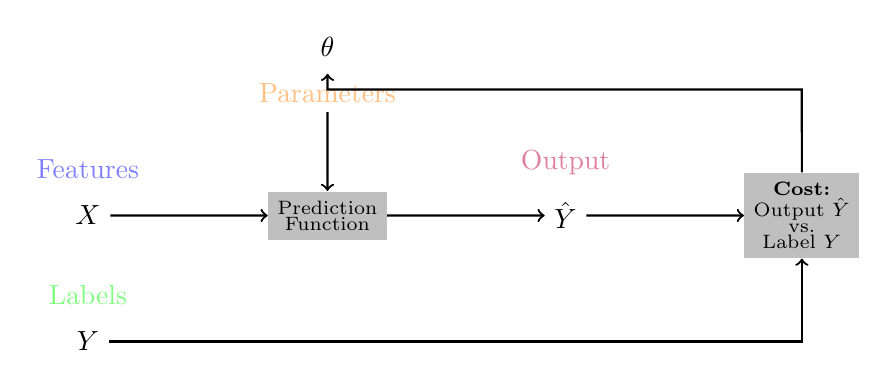
\begin{tikzpicture}[scale=0.8]
    \node (x) at (0, 2) {$X$};
    \node (features) [above=1mm of x] {\color{blue!50}{Features}};
    \node (y) at (0, 0) {$Y$};
    \node (labels) [above=1mm of y] {\color{green!50}{Labels}};
    \node[fill=gray!50,rectangle,right = 2cm of x] (predictionfunction)     {$\substack{\textrm{Prediction} \\ \textrm{Function}}$};
    \node[above = 1cm of predictionfunction] (params)     {\color{orange!50}{Parameters}};
    \node[above = 1mm of params] (theta) {$\theta$};
    \node[right = 2cm of predictionfunction] (yhat) {$\hat Y$};
    \node (output) [above=1mm of yhat] {\color{purple!50}{Output}};
    \node[fill=gray!50,rectangle,right = 2cm of yhat] (cost) {$\substack{\textrm{\textbf{Cost:}} \\ \textrm{Output } \hat Y \\ \textrm{vs.}     \\ \textrm{Label } Y}$};
\draw[->,thick] (x) -- (predictionfunction);
\draw[->,thick] (predictionfunction) -- (yhat);
\draw[->,thick] (yhat) -- (cost);
% Draw a path in two steps and go via a coordinate relative to the first node.
\draw[->,thick] (y) -- node {} ++(2cm,0) -| (cost);
\draw[->,thick] (cost) -- node{} ++(0,2cm) -| (params);
\draw[->,thick] (params) -- (predictionfunction);
\end{tikzpicture}
\end{center}
\label{fig: supervised_ml}
\caption{Overview of supervised machine learning.}
\end{figure}

How about the supervised ML classification task of sentiment analysis? Suppose we're given a tweet that says, ``I'm happy because I'm learning NLP'': and the objective in the task is to predict whether a tweet has a positive or negative sentiment. We'll do this by starting with a training set where tweets with a positive label have a label of unit value, and tweets with a negative sentiment have a label of zero.
To get started building a logistic regression classifier that's capable of predicting sentiments of an arbitrary tweet, we first need to process the raw tweets in our training data set and extract useful features. Then, we will train our logistic regression classifier while minimimizing the cost. Finally, we'll be able to make predictions.

\subsubsection{Representation of Text}
\paragraph{How to represent text as a vector} In order to represent text as a vector, we need to first build a vocabulary. We define the vocabulary $V$ as the \emph{set} of unique words from your input data (e.g. your listing of tweets). To get this listing, we quite literally need to comb through all words from all input data and save every new word that appears in our search.
To represent a tweet as a vector, we can use a one-hot encoding with our vocabulary: i.e. each tweet will be represented with a length $|V|$ vector where elements are binary-valued - a one indicates the word is in the tweet and a zero indicates the absence of a word in a tweet. We call this a \emph{sparse} representation because the number of non-zero entries is relatively small when compared with the number of zero entries. Realize that if we are running a logistic regression, we would require learning $|V| + 1$ parameters which can be problematic for large vocabularies. If not prohibitive, it would make training models take excessive time and making predictions would be expensive.

\paragraph{Negative and positive frequencies} Let's discuss how to generate counts which can be used as features in our logistic regression classifier. Specifically, given a word, we wish to keep track of the number of times that it shows up as the positive class. Given another word, we wish to track how many times that word shows up in the negative class. Using both these counts, we can then extract features and use those features in our logistic regression classifier. Suppose we have the following corpus of tweets:
\begin{verbatim}
I am happy because I am learning NLP
I am happy
I am sad, I am not learning NLP
I am sad
\end{verbatim}
Then our vocabulary is given by
\begin{center}
  \begin{tabular}{c}
    \hline
    Vocabulary \\
    \hline
    I \\
    am \\
    happy \\
    because \\
    learning \\
    NLP \\
    sad \\
    not
  \end{tabular}
\end{center}

For this particular example of sentiment analysis, we only have two sentiments (i.e. two classes): one class is associated with a positive sentiment and the other with a negative sentiment. So, taking your corpus, you'd have a set of two tweets that belong to the positive class, and two tweets which belong to the negative class. Let's calculate the positive frequencies by examining the first two tweets:

\begin{center}
  \begin{tabular}{c c}
    \hline
    Vocabulary & PosFreq(1) \\
    \hline
    I  & 3 \\
    am & 3 \\
    happy & 2 \\
    because & 1 \\
    learning & 1 \\
    NLP & 1 \\
    sad & 0 \\
    not & 0
  \end{tabular}
\end{center}

The same logic applies applies to getting negative frequencies. We can calculate these by examining our last two training examples.


\begin{center}
  \begin{tabular}{c c}
    \hline
    Vocabulary & NegFreq(0) \\
    \hline
    I  & 3 \\
    am & 3 \\
    happy & 0 \\
    because & 0 \\
    learning & 1 \\
    NLP & 1 \\
    sad & 2 \\
    not & 1
  \end{tabular}
\end{center}

So, we can now have an entire table for our corpus, where for each entry in $V$ we associate with it a scalar value \texttt{PosFreq(1)} and another scalar value \texttt{NegFreq(0)}. In practice, we use a Python dictionary \texttt{freqs} mapping from \texttt{(word, class)} $\leadsto$ frequency.

\subsubsection{Feature Extraction with Frequencies} Whereas we previously learned to encode a tweet as a vector of length $|V|$, we will now use our frequency counts to represent each tweet as a vector of length equal to one plus the number of classes in our set of labels. This gives us a much faster speed for our logistic regression classifier. How can we do this, exactly? We represent each tweet as follows:

\begin{align*}
\underbrace{X_m}_{\substack{\textrm{Features of} \\ \textrm{tweet } m}} = \bigg [ \underbrace{1}_{\textrm{Bias}}, \underbrace{\sum_w \texttt{freqs}(w, 1)}_{\substack{\textrm{Sum Pos.} \\ \textrm{Frequences}}}, \underbrace{\sum_w \texttt{freqs}(w, 0)}_{\substack{\textrm{Sum Neg.} \\ \textrm{Frequencies}}} \bigg ]
\end{align*}

I.e. the first feature is a bias unit equal to unit value, the second is the sum of positive frequencies for every unique word on tweet $m$, and the third is the sum of negative frequencies for every unique word on the tweet.
So, to extract the features for this \emph{representation}, we only have to sum frequencies of words, which is straightforward. Let's look at an example: ``I am sad, I am not learning NLP''. The only words in our vocabulary that don't appear in this sentence are ``happy'' and ``because'': if we sum up the \texttt{PosFreq(1)} associated with the remaining words in our vocabulary, i.e. the words that appear in this tweet, we get a scalar value of eight. We do the same for the negative frequencies, and we get a scalar value of eleven. So, we represent ``I am sad, I am not learning NLP'' $\leadsto [1, 8, 11]$.

\subsubsection{Preprocessing} There are two major concepts here: stemming and ``stop words''.
We'll learn how to apply these preprocessing steps to our data.
\paragraph{Stop words}
Stop words are defined as those which don't add significant meaning to the tweets; we \emph{might} also choose to remove punctuation (if we decide it doesn't provide information in our context). In practice, this means comparing our tweet against two sets: one with stop words (in English) and another with punctuation. 

\begin{minipage}{1.0\textwidth}
  \begin{multicols}{2}
      \begin{tabular}{c c}
        \hline
        Stop Words \\
        \hline
        and \\
        is \\
        are \\
        at \\
        has \\
        for \\
        a \\
      \end{tabular}
    \vfill\null \columnbreak  
    \begin{tabular}{c c}
      \hline
      Punctuation \\
      \hline
      , \\
      . \\
      : \\
      ! \\
      `` \\
      ' \\
    \end{tabular}
\end{multicols}
\end{minipage}
In practice the list of stop words and punctuation marks are much larger, but for pedagogical purposes these will serve well.
We might start out with a tweet like
\begin{verbatim}
@YMourri and @AndrewYNg are tuning a GREAT AI Model at https://deeplearning.ai!!!
\end{verbatim}
We then preprocess by stripping stop words ``and'', ``are'', a''at'', and ``a''. The only punctuation that appears in this tweet that's also in our list is the exclamation point(s). We might further decide that tweets should have handles and URLs removed, because these don't add value for the specific task of sentiment analysis. In the end, we end up with a data point that looks like
\begin{verbatim}
tuning GREAT AI model
\end{verbatim}
It's clearly a positive tweet, and a sufficiently good model should be able to classify it. Now that the tweet contains the minimum necessary information, we can perform \emph{stemming} for every word.

\paragraph{Stemming}
Stemming in NLP is simply transforming any word to its base stem, which you could define as the set of characters that are used to construct the words and its derivatives. Let's look at the first word in the example: its stem is ``tun'', since
\begin{center}
  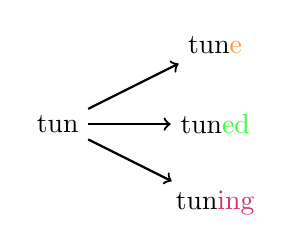
\begin{tikzpicture}
    \node (tun) at (-1,0) {tun};
    \node (tune) at (1, 1) {tun\color{orange!80}{e}};
    \node (tuned) at (1, 0) {tun\color{green!80}{ed}};
    \node (tuning) at (1, -1) {tun\color{purple!80}{ing}};
    \draw[->,thick] (tun) -> (tune);
    \draw[->,thick] (tun) -> (tuned);
    \draw[->,thick] (tun) -> (tuning);
  \end{tikzpicture}
\end{center}

If we were to perform stemming on our entire corpus, the words ``tune'', ``tuned'', and ``tuning'' all get reduced to the stem ``tun''. So, your vocabulary would be significantly reduced in performing this process. You can further reduce the size of the vocabulary without losing valuable information by \emph{lower-casing} every word, e.g. the words ``GREAT'', ``Great'', and ``great'' all get treated as the same word. Perhaps our final preprocessed tweet looks like
\begin{verbatim}
[tun, great, ai, model]
\end{verbatim}

In summary, for our example of sentiment analysis on tweets, we might preprocess as follows:
\begin{enumerate}
\item Eliminate handles and URLs
\item Tokenize the string into words
\item Remove stop words like ``and, is, a, on, etc.''
\item Stemming - or convert every word to its stem. E.g. dancer, dancing,   danced, becomes ``danc''. You can use \href{https://tartarus.org/martin/PorterStemmer/}{Porter Stemmer} to take care of this.
\item Convert all words to lowercase.
\end{enumerate}

As an applied example:
$$
\textrm{I am Happy Because I am learning NLP @deeplearning} \overset{\small \textrm{Preprocessing}}{\longrightarrow} [\texttt{happy, learn, nlp}] \overset{\small \textrm{Feature Extraction}}{\longrightarrow} [1, 4, 2]
$$
where 1 is our bias term, 4 is the sum of positive frequencies, and 2 is the sum of negative frequencies.
In practice, we are given a set of $m$ raw tweets, and so wehave to process them one-by-one to process them into an $m \times 3$ matrix, where each row describes the features for a given tweet.

\begin{equation*}
  \begin{bmatrix}
    1 & X_1^{(1)} & X_2^{(1)} \\
    1 & X_1^{(2)} & X_2^{(2)} \\
    \vdots & \vdots & \vdots \\
    1 & X_1^{(m)} & X_2^{(m)} \\
  \end{bmatrix}
\end{equation*}

The process is simple: (i) build the frequencies dictionary, (ii) initialize the matrix $X$ to match the number of tweets, (iii) go through your sets of tweets and carefully preprocess by deleting stop words, stemming, deleting URLs/handles, and lowercasing, and finally (iv) extract the features by summing up the positive and negative frequencies of each of the tweets.

\begin{python}
freqs = build_freqs(tweets, labels)          # Build frequencies dictionary.
X = np.zeros((m,3))                          # Initialize matrix X.
for i in range(m):                           # For every tweet:
  p_tweet = process_tweet(tweets[i])         #   Process tweet.
  X[i,:] = extract_features(p_tweet, freqs)  #   Extract features.
\end{python}

\subsection{Logistic Regression} Previously, we've learned how to extract features, which we will now use to predict whether a tweet has a positive or negative sentiment. Logistic regression makes use of a \href{https://en.wikipedia.org/wiki/Logistic_function#Mathematical_properties}{sigmoid (or standard logistic) function} which outputs a probability between zero and one. What's the recap from supervised machine learning? Recall figure \ref{fig: supervised_ml}: in the case of logistic regression our prediction function is going to be the standard logistic function:

\[
  h(x^{(i)}, \theta) = \frac{1}{1 + e^{-\theta^T x^{(i)}}}.
\]
where $i$ denotes the observation number. Note that as $\theta^T x^{(i)}$ gets closer and closer to $-\infty$, the denominator of the sigmoid expression blows up and as a result the output values gets closer to zero. Conversely, as the inner product $\theta^T x^{(i)}$ gets closer to $\infty$, the denominator of the sigmoid function approaches unit value and the resulting sigmoid expression evaluates to something near one.
For classification, a threshold is needed, and it is natural to set it at $\frac{1}{2}$. For the logistic function, this threshold occurs when the inner product $\theta^T x^{(i)} = 0$. If the inner product is greater than (or equal to) zero, we classify as positive, else negative.

\subsubsection{Learning Parameters}
\paragraph{How to learn $\theta$?} To train a logistic regression classifier, we need to iterate until we find a set of parameters $\theta$ that minimizes our cost function. Suppose we have a loss that depends only on the parameters $\theta_1, \theta_2$: you might have a cost function that looks like follows, on the left, with the evaluation of the cost function plotted on the right as a function of the number of training iterations:

\begin{minipage}{1.0\textwidth}
  \begin{multicols}{2}
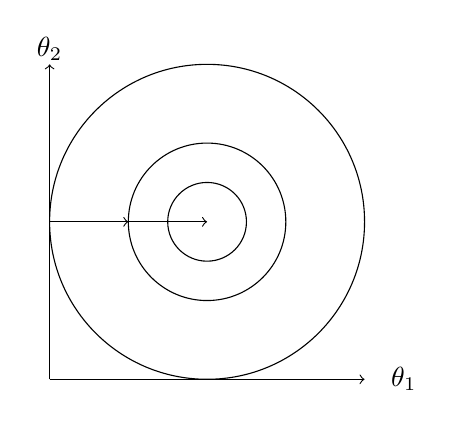
\begin{tikzpicture}[scale=2]
  \draw[->] (-1, -1) to (-1, 1);
  \node at (-1, 1.1) {$\theta_2$};
  \draw[->] (-1, -1) to (1, -1);
  \node at (1.25, -1) {$\theta_1$};
  \draw (0, 0) circle (1cm);   
  \draw (0, 0) circle (.5cm); 
  \draw (0, 0) circle (.25cm); 
  \draw[->] (-1, 0) to (-.5, 0);
  \draw[->] (-.5, 0) to (0, 0);
\end{tikzpicture}
\vfill\null \columnbreak
\begin{tikzpicture}[scale=3]
  \draw[->] (0, 0) to (0, 1.4) node [left] {cost};
  \draw[->] (0, 0) to (2.1, 0) node [right]{\# iterations}; 
  \draw[smooth, domain=0.2:2, color=orange, thick]
    plot (\x,{exp(-\x)}) {};
\end{tikzpicture}
\end{multicols}
\end{minipage}

We might first initialize our parameters $\theta$, then update our parameters in the direction of the \emph{gradient of the cost function}. After a sufficient number of training steps, we will have updated $\theta$ to their optimal values where we are achieving near optimal cost. Let's quickly review this process of gradient descent for logistic regression:

\begin{figure}[h]
\begin{center}
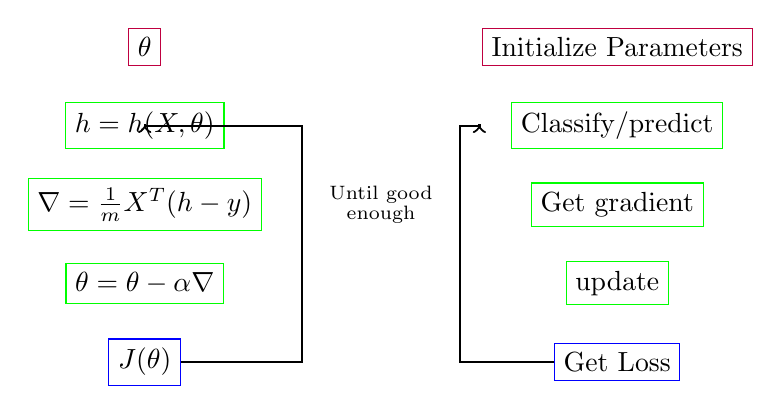
\begin{tikzpicture}
  % Left partition
  \node[draw,rectangle,color=purple] (theta) at (-2, 2) {\color{black}$\theta$};
  \node[draw,rectangle,color=green] (h) at (-2, 1) {\color{black}$h = h(X,\theta)$};
  \node[draw,rectangle,color=green] (gradient) at (-2, 0) {\color{black}$\nabla = \frac{1}{m} X^T (h-y)$};
  \node[draw,rectangle,color=green] (update_eq) at (-2, -1) {\color{black}$\theta = \theta - \alpha \nabla$};
  \node[draw,rectangle,color=blue] (cost) at (-2, -2)   {\color{black}$J(\theta)$};
  \draw[->,thick] (cost) -- ++(2, 0) -- ++(0,3) -| (h);
  % Right partition
  \node[draw,rectangle,color=purple] (init) at (4, 2) {\color{black}Initialize Parameters};
  \node[draw,rectangle,color=green] (classifypredict) at (4, 1) {\color{black}Classify/predict};
  \node[draw,rectangle,color=green] (gradient) at (4, 0) {\color{black}Get gradient};
  \node[draw,rectangle,color=green] (update_eq) at (4, -1) {\color{black}update};
  \node[draw,rectangle,color=blue] (getloss) at (4, -2)   {\color{black}Get Loss};
\draw[->,thick] (getloss) -- ++(-2, 0) -- ++(0,3) -| ++(0.25, 0);

% Middle comment
\node at (1, 0) {$\substack{\textrm{Until good} \\ \textrm{enough}}$};
\end{tikzpicture}
\end{center}
\end{figure}

\subsubsection{Assessing model generalization}
To analyze model fit, we need the following: $(X_{\textrm{val}}, Y_{\textrm{val}}, \theta)$, where we have \emph{validation} data that was set aside during training, and a learned $\theta$ parameter vector. We will compute, for each example in $X_{\textrm{val}}$, the value of $h(\theta, x^{(i)})$ and compare it with our threshold value to make a prediction. In particular, our simple prediction function is given by
\[
  \hat Y_{\textrm{val}} = h(X_{\textrm{val}}, \theta) \geq \frac{1}{2}.
\]

In particular, we will have a vector $h = \begin{bmatrix} h_1 & h_2 & \ldots & h_m \end{bmatrix}$ where e.g. $h_i$ could equal some float in $[0,1]$, which we then convert into a binary label vector by applying our threshold. After building our predictions vector $\hat Y_{\textrm{val}}$, we can compare the predictions with the actual values and evaluate our test-set \emph{accuracy}:

\begin{equation*}
\texttt{Accuracy} = \sum_{i=1}^m \frac{\left(\texttt{pred}^{(i)} == \hat Y_{\textrm{val}}^{(i)}\right)}{m}.
\end{equation*}

This metric gives an estimate of the number of times of logistic regression model will work correctly on unseen data.

\subsubsection{Deriving Gradient Descent for Logistic Regression}
\paragraph{Motivating where cost function comes from} Let's examine the equation for the cost function for logistic regression:

\begin{equation}
  \label{eq: crossentropyloss}
  J(\theta) = -\frac{1}{m} \sum_{i=1}^{m} \left[ y^{(i)} \log h(x^{(i)}, \theta) + (1 - y^{(i)}) \log \left(1 - h(x^{(i)}, \theta)\right)\right].
\end{equation}

The deep learning notes derive this equation in detail in the introduction. Let us briefly recap.
\[
  \Pr(y | x^{(i)}, \theta) = h(x^{(i)}, \theta)y^{(i)}\left(1 - h(x^{(i)}, \theta)\right)^{(1-y^{(i)})}.
\]

We wish to maximize our function $h(\cdot, \theta)$ over the parameter space $\theta$: when $y=0$ we want $(1 - h(x^{(i)}, \theta))$ to be zero, and therefore $h(x^{(i)}, \theta)$ close to one. When $y=1$, we want $h(x^{(i)},\theta) = 1$. To model our entire dataset and not just one observation, we make an assumption of independence to arrive at a joint likelihood:
\[
  L(\theta) = \prod_{i=1}^m h(x^{(i)}, \theta)^{y^{(i)}} \left(1 - h(x^{(i)}, \theta)\right)^{(1 - y^{(i)})}.
\]

Realize that if we ``mess up'' one prediction, we have the potential to ``mess up'' the entire cost function, which is what we want: we want a model that captures the entire dataset, where all datapoints are related. One issue: what happens when $m$ grows? Then $L(\theta) \leadsto 0$, because the expressions
$h(x^{(i)}, \theta)$ and correspondingly $(1 - h(x^{(i)}, \theta)$ are bounded between $(0,1)$.

\paragraph{Optimization}
Using properties of logarithms (that they are monotone and maximizing a function under a monotone transformation doesn't change the optimum, and that they turn multiplication into addition), i.e.
\begin{align*}
  \log(a*b*c) = \log a + \log b + \log c \, \, \, \, \, \textrm{ and } \, \, \, \, \, \log a^b = b \log a.
\end{align*}
We may now rewrite our optimization problem:
\begin{align*}
  \max_{h(x^{(i)}, \theta)} \log L(\theta) &= \log \prod_{i=1}^{m} h(x^{(i)},                                              \theta)^{y^{(i)}} \left(1 - h(x^{(i)}, \theta)\right)^{1 - y^{(i)}} \\
  &= \sum_{i=1}^{m} \log h(x^{(i)}, \theta)^{y^{(i)}} \left(1 - h(x^{(i)},     \theta)\right)^{1 - y^{(i)}} \\
  &= \sum_{i=1}^{m} \log h(x^{(i)}, \theta)^{y^{(i)}}  + \log \left(1 - h(x^{(i)}, \theta)\right)^{1 - y^{(i)}} \\
  &= \sum_{i=1}^{m} y^{(i)} \log h(x^{(i)}, \theta) + (1 - y^{(i)}) \log \left(1 - h(x^{(i)}, \theta)\right)  
\end{align*}

We can then rescale by $\frac{1}{m}$ to get \emph{average} cost. Recall we are maximizing over $h(x^{(i)}, \theta)$ in the equation above, and maximizing an equation is the same as minimizing its negative. Therefore,
\[
  J(\theta) = -\frac{1}{m} \sum_{i=1}^{m} \left[ y^{(i)} \log h(x^{(i)}, \theta) + (1 - y^{(i)}) \log \left(1 - h(x^{(i)}, \theta)\right)\right]. 
\]

A vectorized implementation is given by
\begin{align*}
  h &= g(X\theta) \\
  J(\theta) &= \frac{1}{m} \cdot \left(-y^T \log(h) - \left(1 - y \right)^T \log (1 - h)\right)
\end{align*}

\paragraph{Intuition for loss function of logistic regression}
Now, let's just go over some intuition here. Consider the term on the left-hand side of the parenthesized expression: this is the relevant term in your cost function when your label is 1. The term on the right is relevant when the label is zero. In general, this loss function simply says: the closer the prediction is to the observed label, the smaller the loss incurred. We can plot the cost as a function of our the prediction value for a single training example.

\begin{minipage}{1.0\textwidth}
  \begin{multicols}{2}
    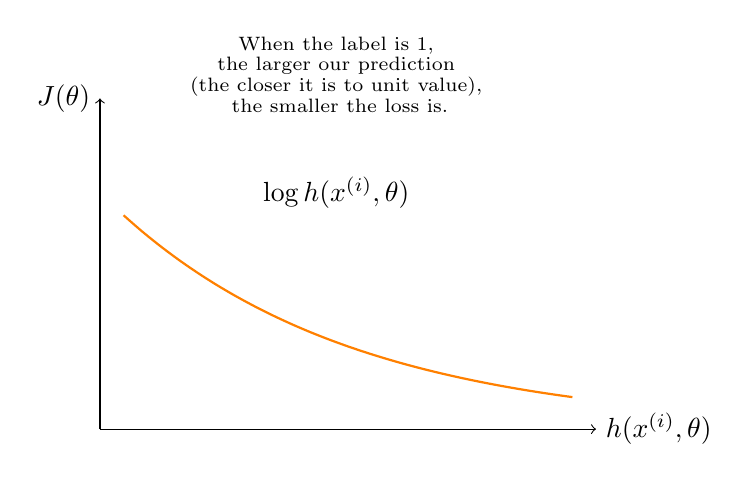
\begin{tikzpicture}[scale=3]
      \draw[->] (0, 0) to (0, 1.4) node [left] {$J(\theta)$};
      \draw[->] (0, 0) to (2.1, 0) node [right]{$h(x^{(i)}, \theta)$}; 
      \draw[smooth, domain=0.1:2, color=orange, thick]
      plot (\x,{exp(-\x)}) {};
      % plot (\x,{-log2(\x/2)}) {};
      \node at (1, 1) {$\log h(x^{(i)}, \theta)$};
      \node at (1, 1.5) {$\substack{\textrm{When the label is 1,} \\ \textrm{the larger our prediction} \\ \textrm{(the closer it is to unit value),} \\ \textrm{ the smaller the loss is.}}$};
    \end{tikzpicture}
    \vfill\null \columnbreak
    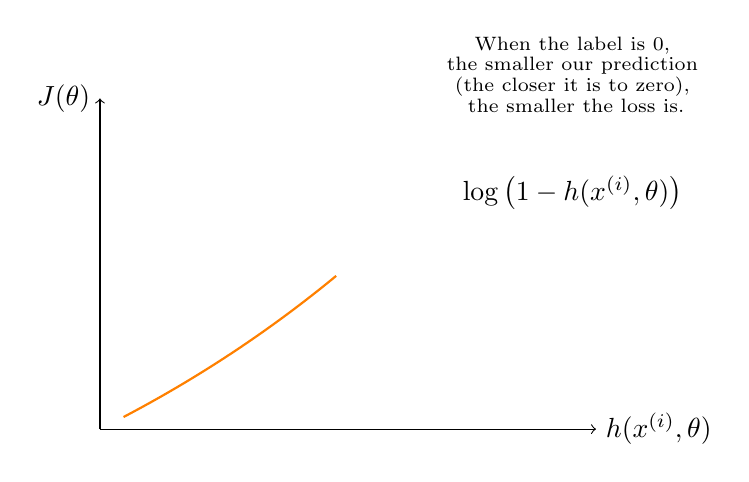
\begin{tikzpicture}[scale=3]
      \draw[->] (0, 0) to (0, 1.4) node [left] {$J(\theta)$};
      \draw[->] (0, 0) to (2.1, 0) node [right]{$h(x^{(i)}, \theta)$}; 
      \draw[smooth, domain=0.1:1, color=orange, thick]
      % plot (\x,{\x^2}) {};
      plot (\x, {exp(\x/2)-1}) {};
      \node at (2, 1) {$\log \left(1 -  h(x^{(i)}, \theta)\right)$};
      \node at (2, 1.5) {$\substack{\textrm{When the label is 0,} \\ \textrm{the smaller our prediction} \\ \textrm{(the closer it is to zero),} \\ \textrm{ the smaller the loss is.}}$};
\end{tikzpicture}
\end{multicols}
\end{minipage}

\newpage
\paragraph{Deriving logistic regression gradient}
The general form of logistic regression is given by

\begin{algorithm}
  \caption{General form of gradient descent}
  \While{not converged, and for all $j$}{
    $\theta_j \gets \theta_j - \alpha \frac{\partial}{\partial \theta_j}     J(\theta)$
  }
\end{algorithm}

We can work out the derivative using partial calculus to fill in the expression further:

\begin{algorithm}
  \caption{Gradient descent for logistic regression}
  \While{not converged, and for all $j$}{
    $\theta_j \gets \theta_j - \frac{\alpha}{m} \sum_{i=1}^m \left(h(x^{(i)}, \theta) - y^{(i)}\right) x_j^{(i)}$
  }
\end{algorithm}

A vectorized implementation is given by
\[
  \theta := \theta - \frac{\alpha}{m} X^T \left(H(X,\theta) - Y\right).
\]

\paragraph{Partial derivative of $J(\theta)$} It'll be helpful to first calculate the derivative of the sigmoid function.
\begin{align*}
  h(x)' &= \left( \frac{1}{1 + e^{-x}} \right)' = \frac{-(1 + e^{-x})'}{(1 + e^{-x})^2} = \frac{-1' - (e^{-x})'}{(1 + e^{-x})^2} = \frac{0 -           (-x)'(e^{-x})}{(1 + e^{-x})^2} = \frac{e^{-x}}{(1 + e^{-x})^2} \\
        &= \left( \frac{1}{1 + e^{-x}} \right) \left( \frac{e^{-x}}{1 + e^{-x}} \right) = h(x) \left( \frac{+1 - 1 + e^{-x}}{1 + e^{-x}} \right) = h(x) \left(\frac{1+e^{-x}}{1+e^{-x}} - \frac{1}{1+e^{-x}}\right) = h(x) (1 - h(x)).
\end{align*}

The above was all for a computation of the derivative of the sigmoid function. But what about the derivative of $h(x^{(i)}, \theta) = \frac{1}{1 + e^{-\theta^T x^{(i)}}}$ with respect to $\theta_j$? Using the chain rule, because of the inner product $\theta^T x^{(i)}$, and applying toward $\theta_j$, we see that the derivative would be
\[
  h(x^{(i)},\theta)\left(1 - h(x^{(i)},\theta)\right) x_j^{(i)}.
\]

Now, we can compute the partial derivative of our loss function with respect to $\theta_j$:

\begin{align*}\frac{\partial}{\partial \theta_j} J(\theta) &= \frac{\partial}{\partial \theta_j} \frac{-1}{m}\sum_{i=1}^m \left [ y^{(i)} log ( h(x^{(i)}, \theta) ) + (1-y^{(i)}) log (1 -  h(x^{(i)}, \theta)) \right ] \\ &= - \frac{1}{m}\sum_{i=1}^m \left [     y^{(i)} \frac{\partial}{\partial \theta_j} log ( h(x^{(i)}, \theta))   + (1-y^{(i)}) \frac{\partial}{\partial                                                                                  \theta_j} log (1 -  h(x^{(i)}, \theta))\right ] \\
                                                           &= - \frac{1}{m}\sum_{i=1}^m \left [     \frac{y^{(i)} \frac{\partial}{\partial \theta_j}  h(x^{(i)}, \theta)}{ h(x^{(i)}, \theta)}   + \frac{(1-y^{(i)})\frac{\partial}{\partial                                                      \theta_j} (1 -  h(x^{(i)}, \theta))}{1 -  h(x^{(i)}, \theta)}\right ] \\
                                                           &= - \frac{1}{m}\sum_{i=1}^m \left [     \frac{y^{(i)} \frac{\partial}{\partial \theta_j}  h(x^{(i)}, \theta)}{ h(x^{(i)}, \theta)}   + \frac{(1-y^{(i)})\frac{\partial}{\partial \theta_j} (1 -  h(x^{(i)}, \theta))}{1                                                              -  h(x^{(i)}, \theta)}\right ] \\
                                                           &= - \frac{1}{m}\sum_{i=1}^m \left [     \frac{y^{(i)}  h(x^{(i)}, \theta) (1 -  h(x^{(i)}, \theta)) \frac{\partial}{\partial \theta_j} \theta^T x^{(i)}}{ h(x^{(i)}, \theta)}   + \frac{- (1-y^{(i)})  h(x^{(i)}, \theta)(1 -  h(x^{(i)}, \theta)) \frac{\partial}{\partial \theta_j} \theta^T x^{(i)}}{1 -  h(x^{(i)},                                                              \theta)}\right ] \\
                                                           &= - \frac{1}{m}\sum_{i=1}^m \left [     \frac{y^{(i)}  h(x^{(i)}, \theta) (1 -  h(x^{(i)}, \theta)) \frac{\partial}{\partial \theta_j} \theta^T x^{(i)}}{ h(x^{(i)}, \theta)}   - \frac{(1-y^{(i)}) h(x^{(i)}, \theta) (1 -  h(x^{(i)}, \theta)) \frac{\partial}{\partial \theta_j} \theta^T x^{(i)}}{1 -  h(x^{(i)},                                                              \theta))}\right ] \\
                                                           &= - \frac{1}{m}\sum_{i=1}^m \left [     y^{(i)} (1 -  h(x^{(i)}, \theta)) x^{(i)}_j                                                              - (1-y^{(i)})  h(x^{(i)}, \theta) x^{(i)}_j\right ] \\
                                                           &= - \frac{1}{m}\sum_{i=1}^m \left [     y^{(i)} (1 -  h(x^{(i)}, \theta)) -                                                              (1-y^{(i)})  h(x^{(i)}, \theta) \right ] x^{(i)}_j \\
                                                           &= - \frac{1}{m}\sum_{i=1}^m \left [     y^{(i)} - y^{(i)}  h(x^{(i)}, \theta) -                                                               h(x^{(i)}, \theta) + y^{(i)}  h(x^{(i)}, \theta) \right ] x^{(i)}_j \\
                                                           &= - \frac{1}{m}\sum_{i=1}^m \left [ y^{(i)} -  h(x^{(i)}, \theta) \right ] x^{(i)}_j    \\
                                                           &= \frac{1}{m}\sum_{i=1}^m \left [  h(x^{(i)},                               \theta) - y^{(i)} \right ] x^{(i)}_j
\end{align*}
The vectorized version is simply given by
\[
  \nabla J(\theta) = \frac{1}{m} \cdot X^T \left( H(X, \theta) - Y \right).
\]

\section{Sentiment Analysis with Naive Bayes}\vspace{.1pt} \hrule height 2pt \smallskip \renewcommand{\arraystretch}{1}% Tighter
\subsection{Probability and Bayes Rule} Imagine you have an extensive corpus of tweets that can be categorized as either positive or negative, but not both.


\begin{minipage}{1.0\textwidth}
\begin{multicols}{2}
  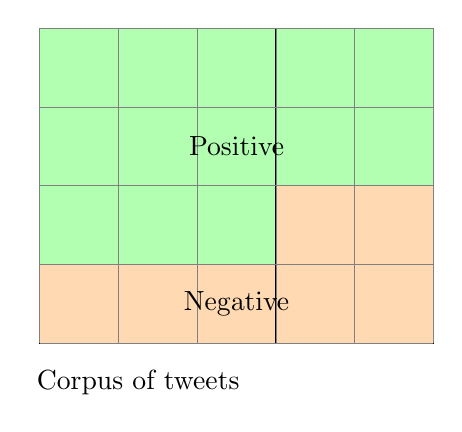
\begin{tikzpicture}
    \draw[fill=green!30] (0, 1) rectangle (3, 4);
    \draw[fill=orange!30] (0, 0) rectangle (3, 1);
    \draw[fill=orange!30] (3, 0) rectangle (5, 2);
    \draw[fill=green!30] (3, 2) rectangle (5, 4);
    \draw[step=1cm, gray, very thin] (0, 0) grid (5, 4);
    \node (neg) at (2.5, 0.5) {Negative};
    \node (pos) at (2.5, 2.5) {Positive};
    \node at (1.25, -0.5) {Corpus of tweets};
  \end{tikzpicture}
  \vfill\null \columnbreak
  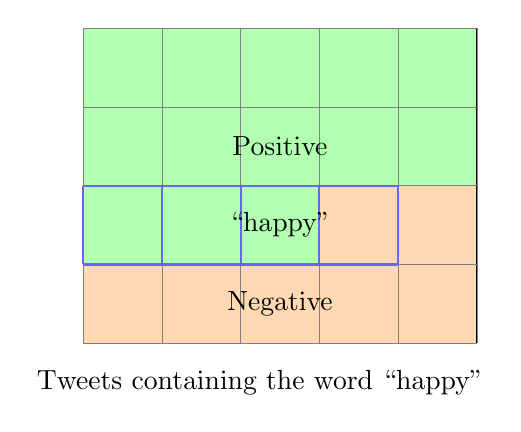
\begin{tikzpicture}
    \draw[fill=green!30] (0, 1) rectangle (3, 4);
    \draw[fill=orange!30] (0, 0) rectangle (3, 1);
    \draw[fill=orange!30] (3, 0) rectangle (5, 2);
    \draw[fill=green!30] (3, 2) rectangle (5, 4);
    \draw[step=1cm, gray, very thin] (0, 0) grid (5, 4);
    \node (neg) at (2.5, 0.5) {Negative};
    \node (pos) at (2.5, 2.5) {Positive};
    \draw[step=1cm, blue!60, thick] (0, 1) grid (4, 2);
    \node (happy) at (2.5, 1.5) {``happy''};
    \node at (2.25, -0.5) {Tweets containing the word ``happy''};
  \end{tikzpicture}
\end{multicols}
\end{minipage}

Within this corpus, observe that the word ``happy'' is sometimes associated with a positive sentiment, but also sometimes with a negative sentiment! How can this happen? Let's explore the situation using probabilities.

\paragraph{Intro probability} Suppose we define an event $A$ as a positive tweet. Then, $\Pr(A) = \Pr(\textrm{Positive}) = \frac{N_{\textrm{pos}}}{N}$, i.e. the ratio between the number of positive-sentiment tweets relative to the total number of tweets observed in our data. In our example above, it comes out $\frac{13}{20}$.\footnote{Of course, because tweets can only be positive or negative but not both, the probability of a negative tweet is simply the complement, i.e. $\Pr(\textrm{Negative}) = 1 - \Pr(\textrm{Positive})$ which in our example happens to be $\frac{7}{20}$.} Let's define an event $B$ as a tweet containing the word ``happy''. In our examples above, this happens to be four, i.e. $\Pr(B) = \Pr(\textrm{``happy''}) = \frac{N_{\textrm{happy}}}{N}$ is $\frac{4}{20}$. Building on this, $\Pr(A \land B) = \Pr(A,B)$ which happens to be $\frac{3}{20}$ in our pictorial example above.

\paragraph{Deriving Bayes rule} What if instead of the entire corpus, we only consider tweets that contain the word ``happy''? $\Pr(A|B) = \Pr(\textrm{Positive} | \textrm{``happy''}) = \frac{3}{4}$ in our example. But we can also do the same thing for positive tweets, i.e.
\[
  \Pr(B|A) = \Pr(\textrm{``happy''} | \textrm{Positive}) = \frac{3}{13}.
\]

There are two equivalent ways of thinking about conditional probabilities:
\begin{figure}[h]
  \begin{center}
    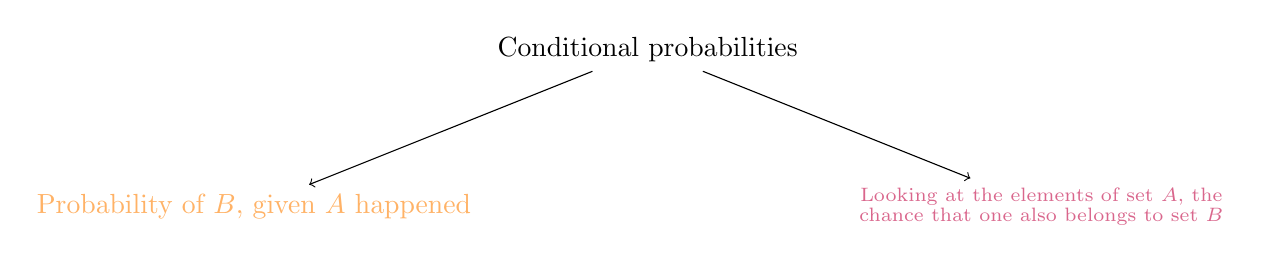
\begin{tikzpicture}
      \node (cp) at (0, 0) {Conditional probabilities};
      \node (l) at (-5, -2) {\color{orange!60} Probability of $B$, given $A$         happened};
      \node (r) at (5, -2) {\color{purple!60} $\substack{\textrm{Looking at the elements of set } A, \textrm{ the} \\ \textrm{chance that one also belongs to set } B}$};
\draw[->] (cp) -- (l);
\draw[->] (cp) -- (r);
    \end{tikzpicture}
  \end{center}
\end{figure}

So, in our context:
\begin{equation}
  \label{eq: bayes1}
  \Pr(\textrm{Positive} | \textrm{``happy''}) = \frac{\Pr(\textrm{Positive} \land \textrm{``happy''})}{\Pr(\textrm{``happy''})}.
\end{equation}

And by symmetry:
\begin{equation}
  \label{eq: bayes2}
  \Pr(\textrm{``happy''} | \textrm{Positive}) = \frac{\Pr(\textrm{``happy''} \land \textrm{Positive})}{\Pr(\textrm{Positive})}.
\end{equation}

Realize that the intersection operation between two events is symmetric, i.e. that the numerator in equations \ref{eq: bayes1} and \ref{eq: bayes2} are identical. Therefore,
\begin{equation}
  \label{eq:bayesrulederivation}
  \Pr(\textrm{Positive} | \textrm{``happy''}) = \Pr(\textrm{``happy''} | \textrm{Positive}) \times \frac{\Pr(\textrm{Positive})}{\Pr(\textrm{``happy''})}.
\end{equation}
This is an expression of Bayes rule in the context of the sentiment analysis problem. More generally: Bayes rule specifies that $\Pr(X|Y) = \Pr(Y|X) \times  \frac{\Pr(X)}{\Pr(Y)}$.

\subsection{Naive Bayes}
\label{sec: naivebayes}
Naive Bayes is often a ``very good, quick, and dirty baseline'' for many text classification tasks; it's an example of supervised machine learning and as such shares many similarities with logistic regression. It's called Naive because it makes the assumption that the features you're using for classification are all independent, which in reality is \emph{rarely} the case. As per usual, we start with two corpora: one for the positive tweets and one for the negative tweets:

\begin{minipage}{1.0\textwidth}
  \begin{multicols}{2}
    \begin{center}
  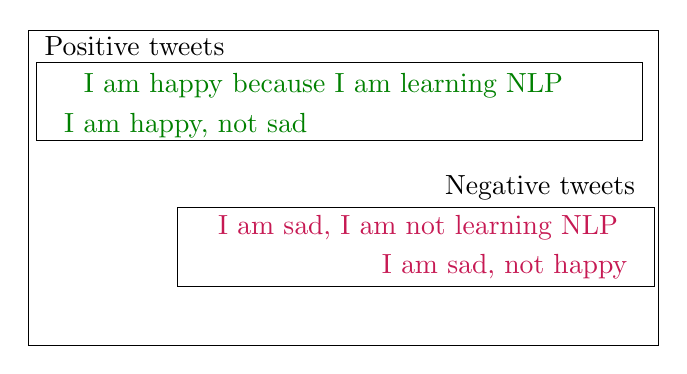
\begin{tikzpicture}
    \draw (0, 2) rectangle (8, -2);
    \node at (1.35, 1.8) {Positive tweets};
    \node at (3.75, 1.3) {\color{green!50!black}I am happy because I am learning NLP};
    \node at (2.00, 0.8) {\color{green!50!black}I am happy, not sad};
    \draw (0.1, 0.6) rectangle (7.8, 1.6);
    \node at (6.5, 0) {Negative tweets};
    \node at (4.95, -0.5) {\color{purple!90} I am sad, I am not learning NLP};
    \node at (6.05, -1) {\color{purple!90} I am sad, not happy};
    \draw (1.9, -1.25) rectangle (7.95, -0.25);
  \end{tikzpicture}
\end{center}
\vfill\null \columnbreak
\begin{tabular}{c c c}
  \hline
  word & {\color{green!50!black} Pos} & {\color{purple!90} Neg} \\
  \hline
  I & 3 & 3 \\
  am & 3 & 3 \\
  happy & 2 & 1 \\
  because & 1 & 0 \\
  learning & 1 & 1 \\
  NLP & 1 & 1 \\
  sad & 1 & 2 \\
  not & 1 & 2 \\
  \hline
  $N_{\textrm{class}}$ & 13 & 13
\end{tabular}
\end{multicols}
\end{minipage}

The above word frequencies table is the backbone input to our naive bayes algorithm: it allows us to compute conditional probabilities. E.g. $\Pr(\textrm{I} | \textrm{Pos}) = \frac{3}{13}$. We can do this for each word in our vocabulary, i.e. compute the conditional probability of it appearing in each class. Notice that if you sum over the probabilities for a particular class, you get 1.

\begin{center}
\begin{tabular}{c c c}
  \hline
  word & {\color{green!50!black} Pos} & {\color{purple!90} Neg} \\
  \hline
  I & $\frac{3}{13}$ & $\frac{3}{13}$ \\
  am & $\frac{3}{13}$ & $\frac{3}{13}$ \\
  {\color{green!50!black} happy} & $\frac{2}{13}$ & $\frac{1}{13}$ \\
  because & $\frac{1}{13}$ & 0 \\
  learning & $\frac{1}{13}$ & $\frac{1}{13}$ \\
  NLP & $\frac{1}{13}$ & $\frac{1}{13}$ \\
  {\color{purple!90}sad} & $\frac{1}{13}$ & $\frac{2}{13}$ \\
  {\color{purple!90}not} & $\frac{1}{13}$ & $\frac{2}{13}$ \\
  \hline
  Sum & 1 & 1
\end{tabular}
\end{center}

Let's inspect some of the entries: notice that for a few words in the vocabulary, their conditional probabilities of appearing in either class are (nearly) identical: words that are equally probable don't add anything to the sentiment. On the other hand, words like {\color{green!50!black} happy}, or {\color{purple!90} sad, not} are ``power'' words which tend to express one sentiment or another. These words carry a lot of weight in determining your tweet sentiments. As a separate note, examine the word \texttt{because}: it only appears in the positive corpus, and so its conditional probability for the negative class is zero: when this happens we have no way of comparing between the two corpora which will become a problem for subsequent calculations. We'll see how we can ``smooth'' our probability function.

Suppose we get a new tweet, ``I am happy today; I am learning.'' and we want to classify its sentiment. We use the following expression:
\[
  \prod_{i=1}^{m} \frac{\Pr(w_i | \textrm{pos})}{\Pr(w_i|\textrm{neg})}
\]

So, for our tweet example, we have (word by word, and skipping ``today'' because it doesn't appear in our vocabulary):
\[
  \frac{\frac{3}{13}}{\frac{3}{13}} \times \frac{\frac{3}{13}}{\frac{3}{13}} \times \frac{\frac{2}{13}}{\frac{1}{13}} \times \frac{\frac{3}{13}}{\frac{3}{13}} \times \frac{\frac{3}{13}}{\frac{3}{13}} \times \frac{\frac{1}{13}}{\frac{1}{13}} = \frac{2}{13} {\color{green!50!black} > 1}.
\]

Because the ratio is greater than unit value, we conclude that overall the sentiment of the tweet is positive.

\paragraph{Laplacian smoothing} This is a technique we use to avoid probabilities being identically zero. Typically, the expression used to calculate the conditional probability of a word, given the class, is
\[
  \Pr(w_i | \textrm{class}) = \frac{\texttt{freq}(w_i, \textrm{class})}{N_{\textrm{class}}} \hspace{35pt} \textrm{class} \, \in \, \{\textrm{Positive}, \textrm{Negative}\}
\]
where $N_{\textrm{class}} = \textrm{ frequency of all words in class}$. Laplacian smoothing does the following; supposing $|V|$ is the number of unique words in the vocabulary
\begin{equation}
  \label{eq: laplaciansmoothing}
  \Pr(w_i | \textrm{class}) = \frac{\texttt{freq}(w_i, \textrm{class}) + 1}{N_{\textrm{class}} + |V|}.  
\end{equation}

By adding a one to our numerator, we ensure the expression is non-zero. However, this is not correctly normalized by $N_{\textrm{class}}$, and so we add a new term to the denominator $|V|$; this ensures the probabilities all sum to one. E.g. in our example table in section \ref{sec: naivebayes} describing positive and negative word frequencies in our corpora of tweets, we can use this to compute
\[
  \Pr(\textrm{I} | \textrm{Pos}) = \frac{3+1}{13+8}.
\]
We can apply Laplacian smoothing to every entry in our table and end up with a new table of conditional probabilities where the column-sums are unit valued.
Notice that if we apply this technique to the word ``because'' in our example, and specificially for the negative class, that $\Pr(\textrm{because} | \textrm{Negative}) = \frac{0 + 1}{13 + 8} > 0$ which solved our original problem of getting a divide by zero in the formula for Naive Bayes $\prod_{i=1}^m \frac{\Pr(w_i | \textrm{Pos})}{\Pr(w_i | \textrm{Neg})}$.

\paragraph{Log likelihoods} Words can have many shades of emotional meaning, but for the purpose of sentiment classification they can be simplified into three categories: neutral, positive, and negative. A word can be taxonomized according to its conditional probabilities. We simply calculate for each word
\[
  \textrm{ratio}(w_i) = \frac{\Pr(w_i | \textrm{{\color{green!50!black}\textrm{Pos}}})}{\Pr(w_i | {\color{purple!90} \textrm{Neg}})} \approx \frac{\texttt{freq}(w_i, {\color{green!50!black} 1}) + 1}{\texttt{freq}(w_i, {\color{purple!90} 0}) + 1}.
\]

If this ratio is identically unit valued, the word is neutral. Words that are more positive tend to have higher ratios (larger than one), and words that are more negative tend to have lower ratios (less than one). Observe that the ratio can lie in $[0, \infty)$.

It turns out that in our previous formulation of Naive Bayes, we assumed balanced class sizes. The correct formula for the likelihood includes the prior ratio, which becomes important for unbalanced datasets (where e.g. the number of positive and negative tweets is not equal):
\begin{equation}
  \label{eq: completenaivebayeswithprior}
  \frac{\Pr(\textrm{Pos})}{\Pr(\textrm{Neg})} \prod_{i=1}^{m} \frac{\Pr(w_i | \textrm{pos})}{\Pr(w_i|\textrm{neg})}  
\end{equation}

Recognize that this computation involves the product of many probabilities that lie in $(0,1]$, and we run the risk of numerical underfluw if the number returned ``is so small it can't be stored on your device''. There is a nice mathematical trick that avoids this pitfall, and that's to use properties of logarithms: $\log(a \times b) = \log (a) + \log (b)$.
\[
\log  \frac{\Pr(\textrm{Pos})}{\Pr(\textrm{Neg})} \prod_{i=1}^{m} \frac{\Pr(w_i | \textrm{pos})}{\Pr(w_i|\textrm{neg})}  \leadsto \underbrace{\log \frac{\Pr(\textrm{Pos})}{\Pr(\textrm{Neg})}}_{\textrm{log prior}} + \underbrace{\sum_{i=1}^{m} \log \frac{\Pr(w_i | \textrm{Pos})}{\Pr(w_i | \textrm{Neg})}}_{\textrm{log likelihood}}.
\]
Let $\lambda(w) = \log \frac{\Pr(w | \textrm{Pos})}{\Pr(w | \textrm{Neg})}$; we calculate this for each word in our vocabulary. Realize that neutral words (i.e. ones where $\Pr(w | \textrm{Pos}) = \Pr(w | \textrm{Neg})$) have $\lambda(w) = \log(1) = 0$. A positive sentiment is indicated by $\lambda(w) > 0$, and correspondingly $\lambda < 0$ indicates a negative sentiment. By using logarithms, we can reduce the risk of numerical underflow.
Realize that our log-likelihood term can be expressed as $\sum_{i=1}^{m} \log \frac{\Pr(w_i | \textrm{Pos})}{\Pr(w_i | \textrm{Neg})} = \sum_{i=1}^m \lambda(w_i) \in (-\infty, \infty)$; we emphasize that our decision boundary is zero with our log-likelihood formula.

\paragraph{Training Naive Bayes} In the context of Naive Bayes, ``train'' means something different than in logistic regression or deep learning: there's no gradient descent; we're just counting word frequencies in a corpus. There are five steps for training a Naive Bayes model:

\begin{enumerate}
\item Collect and annotate corpus (e.g. with positive and negative tweets)
\item Preprocessing (e.g. $\texttt{process\_tweet}(\textrm{tweet}) \leadsto [w_1, w_2, \ldots, ]$)
    \begin{itemize}
    \item Lowercase
    \item Remove punctuation, urls, names, etc.
    \item Remove stop words
    \item Stemming
    \item Tokenize sentences
  \end{itemize}
\item Compute word counts, i.e. $\texttt{freq}(w, \textrm{class})$ and   $N_{\textrm{class}}$.
\item Apply Laplacian smoothing to compute $\Pr(w | \textrm{class}) = \frac{\texttt{freq}(w, \textrm{class}) + 1}{N_{\textrm{class}} +   |V_{\textrm{class}}|}$.
\item Calculate $\lambda(w) = \log \frac{\Pr(w | \textrm{Pos})}{\Pr(w |     \textrm{Neg})}$.
\item Get the log-prior, which involves first counting $D_{\textrm{Pos}} = $ number of positive tweets and $D_{\textrm{Neg}} = $ number of negative tweets, whereby $\log \textrm{ prior } = \log \frac{D_{\textrm{Pos}}}{D_{\textrm{Neg}}}$.\footnote{If the dataset is balanced, the log-prior is zero since $D_{\textrm{Pos}} = D_{\textrm{Neg}}$ and $\log(1) = 0$.}
\end{enumerate}

\paragraph{Testing Naive Bayes} Once you've trained your model, you test it by taking the conditional probabilities derived and using them to predict the sentiments of new unseen tweets. We can evaluate model performance using test set accuracy. In particular, suppose we are given a tweet ``I passed the NLP interview!'', and then after preprocessing we end up with $[\textrm{I, pass, the, NLP, interview}]$. We then look up our $\lambda(w)$'s that were calculated when we ``trained'' our model and compute the score, i.e. the log-prior plus log-likelihood for the unseen test case and compare it to our threshold (of zero). The values of the words that aren't in our vocabulary are treated as neutral (i.e. zeros) and do not contribute to the final score (likelihood) of the unseen word: $\texttt{pred} = \mathbbm 1_{\texttt{score} > 0}$. If we are given a bunch of unseen words, i.e. data set aside during training ($X_{\textrm{val}}, Y_{\textrm{val}}$), we (i) compute $\texttt{score} = \texttt{predict}(X_{\textrm{val}}, \lambda, \texttt{log-prior})$ and then (ii) predict $\texttt{pred} = \mathbbm 1_{\texttt{score} > 0}$, and then (iii) compute test accuracy given by $\frac{1}{m} \sum_{i=1}^m \left(\texttt{pred}_i   == Y_{\textrm{val}_i}\right)$.

\paragraph{Applications of Naive Bayes} There's more we can do than just sentiment analysis. For example, we could do author identification: if you had two large corpora each written by different authors, you could train the model to recognize whether a document was written by one author or the other. Or, if you had some works by Shakespeare and some works by Hemmingway, you could calculate the $\lambda$ for each word to predict how likely a new word is to be used by Shakespeare or alternatively Hemmingway. Another common use is spam filtering: $\frac{\Pr(\textrm{spam} | \textrm{email})}{\Pr(\textrm{non-spam}|\textrm{email})}$. One of the earliest applications of Naive Bayes was to filter between relevant and irrelevant documents in a database. I.e. given a set of keywords in a query, in this case, you can calculate the likelihood of the documents given the query:
\[
  \Pr(\textrm{document}_k | \textrm{query}) \propto \prod_{i=0}^{|\textrm{query}|} \Pr(\textrm{query}_i | \textrm{document}_k).
\]
Then, we have a decision rule that suggests retrieval if $\Pr(\textrm{document}_k | \textrm{query}) > \textrm{threshold}$, and then \emph{sort} the documents based on their likelihoods; perhaps we choose to keep the first $m$ results or ones with a likelihood above a certain threshold. Lastly, we can also use Naive Bayes for word disambiguation, i.e. breaking words down for contextual clarity. Consider that you have two possible interpretations of a given word within a text: let's say you don't know if the word ``bank'' in a text is referring to the bank of a river or a financial institution. To disambiguate your word, calculate the score of the document: $\frac{\Pr(\textrm{river} | \textrm{text})}{\Pr(\textrm{money} |   \textrm{text})}$.

\subsubsection{Assumptions of Naive Bayes} Naive Bayes is a very simple model: it doesn't involve setting any parameters. The method is called ``naive'' because of the assumptions it makes about the data. The first assumption is independence between predictors within each class, and the second has to do class (im)-balance with your validation sets. Let's explore each in detail and how they can affect our results.

\paragraph{Independence} To illustrate what independence between features looks like, lets consider the following example:
\begin{verbatim}
It is sunny and hot in the Sahara Desert.
\end{verbatim}
Naive Bayes assumes the words in a piece of text are independent of one another, but as you can see this is not always the case: the words ``sunny'' and ``hot'' often appear together as they do in this example. When taken together, they might also be related to the thing they're describing like a beach or a desert; so the words in a sentence aren't really independent of one another. But, Naive Bayes assumes that they are. The implication is that we could end up under \emph{or} over estimating the conditional probabilities of individual words. E.g. if your task was to complete the sentence: ``It's always cold and snowy in \{blank\}'', then Naive Bayes might assign equal probability to the words spring, summer, fall, and winter even though from the context winter is the most likely candidate.\footnote{More sophisticated methods can deal with this issue.}

\paragraph{Distribution of training data} A good data set will contain the same proportion of (e.g. positive and negative) classes as a random sample would. However, most available annotated corpora are artificially balanced. E.g. in a real tweet stream a positive tweet is more likely to be sent than a negative tweet. Part of this has to do with platform decisions to perhaps ban content that is inappropriate or contains offensive vocabulary. Assuming that reality behaves as your training corpus could result in a very optimistic \emph{or} pessimistic model.

\subsubsection{Error Analysis} No matter what NLP method you use, you'll one day find yourself faced with an error, e.g. a missclassified sentence. How can we analyze such errors? Let's consider some possible errors in the model prediction that can be caused by:
\begin{itemize}
\item Removing punctuation and stop words -- semantic meaning can be lost in the preprocessing step.
\item Word order -- can affect the meaning of a sentence.
\item Adversarial attacks -- language quirks can confuse Naive Bayes classifiers.
\end{itemize}

\paragraph{Removing punctuation}
Let's consider an example tweet: ``My beloved grandmother :(''. The sad face punctuation in this case is \emph{very} important to the sentiment of the tweet because it tells you what's happening; but, if we remove punctuation then the processed tweet will leave behind a different (positive) sentiment. After processing, we may end up with $[\textrm{belov, grandmoth}]$ which appear positive in nature.

\paragraph{Removing (stop) words}
It's not just about punctuation either, consider as an example ``this is not good, because your attitude is not even close to being nice''. If we remove stop words, we're left with $[\textrm{good, attitude, close, nice}]$. From this set of words, any classifier would infer that the sentiment is positive. There are techniques we will learn about later to handle ``nots'' and word-order. For now, the takeaway is to look at the processed data to make sure your model can get an accurate read.

\paragraph{Word order}
The input pipeline isn't the only source of trouble. E.g. consider the following two tweets:

\begin{verbatim}
I am happy because I did not go.
I am not happy because I did go.
\end{verbatim}

The first is purely positive, the latter is negative. In this case, the ``not'' is important to the sentiment but gets missed by the Naive Bayes classifier: word order can be as important as spelling.

\paragraph{Adversarial attacks}
Lastly, let's discuss adversarial attacks which essentially describe a language phenomenon like sarcasm, irony, and euphemism. Humans pick these up quickly but machines are terrible at it. The tweet, ``This is a ridiculously powerful movie. The plot was gripping and I cried right through until the ending'' contains a somewhat positive movie review, but pre-processing might suggest otherwise. I.e. if we pre-process, you'll get a list of mostly negative words, but these words were in fact used to describe a movie that the author enjoyed. Applying Naive Bayes to this list of words would yield a negative score, unfortunately.

\section{Vector Space Models}\vspace{.1pt} \hrule height 2pt \smallskip \renewcommand{\arraystretch}{1}% Tighter
\subsection{Motivating Vector Space Models}
Let's talk about vector spaces, and what types of information vectors can encode. We'll talk about vector space models, their advantages, and some applications.

Suppose you have two questions:
\begin{verbatim}
Where are you heading?
Where are you from?
\end{verbatim}

The sentences are identical but for the last word. However, the meaning is entirely different. On the other hand, the two questions:
\begin{verbatim}
What is your age?
How old are you?
\end{verbatim}
contain no overlapping words but have identical meaning. Vector space models can identify similarity even when sentences don't share common words; they can also be used for answering paraphrasing, and summarization. One advantage of vector space models is they allow us to capture dependencies between words. E.g.
\begin{verbatim}
You eat cereal from a bowl.
You buy something and someone else sells it.
\end{verbatim}
In the first sentence, the words \emph{cereal} and \emph{bowl} are related (we're eating one thing out of the other). In the second sentence, the latter half of it depends on the first half. Vector space models can capture this and many other types of relationships among different sets of words. When using a vector space models, the way that representations are made are by identifying the \emph{context} around each word in the text, and this captures the relative meaning. ``You shall know a word by the company it keeps'' (John Firth).

\subsection{Word by Word and Word by Doc}
Let's discuss how to construct vectors based off of a co-occurrence matrix. Depending on the task you're trying to solve, you can have several possible designs.

\paragraph{Word by word} To get a vector space model using a word by word design, you'll make a co-occurrence matrix and extract vector representations for the words in your corpus. We'll also discuss how to find relationships between words and vetors, also known as their similarity. We define the \textbf{co-occurrence} of two different words as the number of times they occur together within a certain distance $k$. E.g. suppose our corpus has the following two sentences:
\begin{verbatim}
I like simple data.
I prefer simple raw data.
\end{verbatim}
Then, the row of the co-occurrence matrix corresponding to the word \texttt{data} with a value $k = 2$ would be populated with the following values:

  \begin{table}[h]
    \begin{center}
      \begin{tabular}{l c c c c}
        & simple & raw & like & I \\
        \hline
        data & 2 & 1 & 1 & 0 \\
        \hline
      \end{tabular}
        \caption{The word ``data'' appears within distance one of the word ``simple'' in the first sentence, and within distance two of the word simple in the second example. Both of these are within our tolerance of $k=2$, so the word by word co-occurrence entry for ``data'' and ``simple'' in this example is the value 2. We can proceed to compare the word ``data'' with other words appearing in our vocabulary, populating a representation that is based on word by word co-occurrence counts within a certain window size.}
  \end{center}
\end{table}

With a word by word design, you get a representation with $|V|$ entries, where $V$ is our vocabulary.

\paragraph{Word by document} With a word by document design, you'll count the number of times that words from your vocabulary appear in documents that belong to specific categories.

\begin{center}
  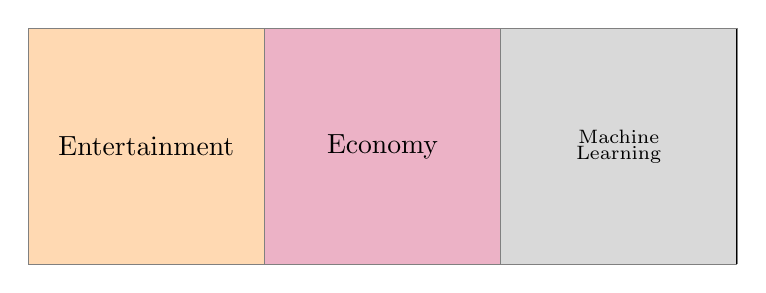
\begin{tikzpicture}[scale=3]
    \draw[fill=orange!30] (0, 0) rectangle (1, 1);
    \draw[fill=purple!30] (1, 0) rectangle (2, 1);
    \draw[fill=gray!30] (2, 0) rectangle (3, 1);
    \draw[step=1cm, gray, very thin] (0, 0) grid (3, 1);
    \node at (0.5, 0.5) {Entertainment};
    \node at (1.5, 0.5) {Economy};
    \node at (2.5, 0.5) {$\substack{\textrm{Machine}\\ \textrm{Learning}}$};
  \end{tikzpicture}
\end{center}

Here, we'd count the number of times that our words appear in the document that belong to each of the three categories. In this example, suppose that the word data appears 500 times in documents from your corpus related to entertainment, 6,620 times in economy documents, and 9,320 in documents related to machine learning. The word film might appear in each document's category 7,000, 4,000, and 1,000 times respectively.

  \begin{table}[h]
    \begin{center}
      \begin{tabular}{l c c c}
        & Entertainment & Economy & $\substack{\textrm{Machine}\\ \textrm{Learning}}$ \\
        \hline
        data & 500 & 6620 & 9320 \\
        film & 7000 & 4000 & 1000 \\
        \hline
      \end{tabular}
    \end{center}
  \end{table}

Once you've constructed representations for multiple sets of documents or words, you'll get your vector space. For example, we could take a representation for the \emph{words} ``data'' and ``film'' by looking at the rows of the table (or matrix). However, we can also get a representation for each \emph{category} of document type by looking at the columns! In our toy example, the vector space will have two dimensions: the number of times that the words ``data'' and ``film'' appear on the type of document.

\begin{figure}[h]
\begin{center}
  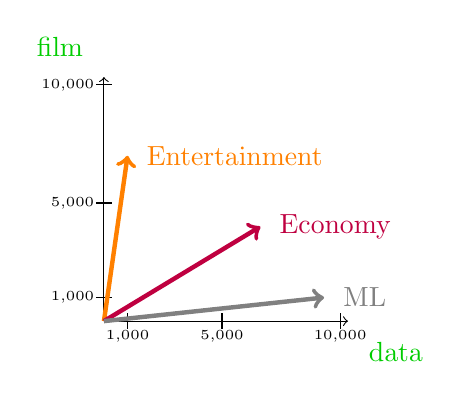
\begin{tikzpicture}
    \draw[->] (0, 0) -- (3.1, 0) node[below right=2mm,color=green!80!black] {data};
    \draw[->] (0, 0) -- (0, 3.1) node[above left=2mm,color=green!80!black] {film};
    % x-axis ticks
    \draw[-] (1.5, -0.1) -- (1.5, 0.1) node[below=1mm] {\tiny 5,000};
    \draw[-] (0.3, -0.1) -- (0.3, 0.1) node[below=1mm] {\tiny 1,000};
    \draw[-] (3.0, -0.1) -- (3.0, 0.1) node[below=1mm] {\tiny 10,000};
    % y-axis ticks
    \draw[-] (-0.1, 1.5) -- (0.1, 1.5) node[left=1mm] {\tiny 5,000};
    \draw[-] (-0.1, 0.3) -- (0.1, 0.3) node[left=1mm] {\tiny 1,000};
    \draw[-] (-0.1, 3.0) -- (0.1, 3.0) node[left=1mm] {\tiny 10,000};
    \draw[->,ultra thick, orange] (0, 0) -- (0.3, 2.1) node[right=1mm] {\color{orange} Entertainment};
    \draw[->,ultra thick, purple] (0, 0) -- (1.986, 1.2) node[right=1mm] {\color{purple} Economy};
    \draw[->,ultra thick, gray] (0, 0) -- (2.796, 0.3) node[right=1mm] {\color{gray} ML};
\end{tikzpicture}
\end{center}
\caption{In this vector representation, the document categories Economy and Machine Learning are more similar to each other than they are to entertainment. Measures of similarity include angle (cosine similarity) and distance (Euclidean, for example).}
\end{figure}

\subsection{Distance and Similarity Metrics}
\paragraph{Euclidean distance}
Euclidean distance is a similarity metric: it identifies how far apart two points (or vectors) are from each other. 

\begin{figure}[h]
\begin{center}
  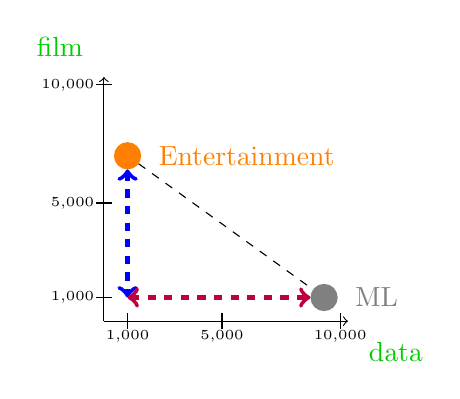
\begin{tikzpicture}
    \draw[->] (0, 0) -- (3.1, 0) node[below right=2mm,color=green!80!black] {data};
    \draw[->] (0, 0) -- (0, 3.1) node[above left=2mm,color=green!80!black] {film};
    % x-axis ticks
    \draw[-] (1.5, -0.1) -- (1.5, 0.1) node[below=1mm] {\tiny 5,000};
    \draw[-] (0.3, -0.1) -- (0.3, 0.1) node[below=1mm] {\tiny 1,000};
    \draw[-] (3.0, -0.1) -- (3.0, 0.1) node[below=1mm] {\tiny 10,000};
    % y-axis ticks
    \draw[-] (-0.1, 1.5) -- (0.1, 1.5) node[left=1mm] {\tiny 5,000};
    \draw[-] (-0.1, 0.3) -- (0.1, 0.3) node[left=1mm] {\tiny 1,000};
    \draw[-] (-0.1, 3.0) -- (0.1, 3.0) node[left=1mm] {\tiny 10,000};
    \node[draw,circle,fill,orange] (e) at (0.3, 2.1) {};
    \node[draw,circle,fill,gray] (ml) at (2.796, 0.3) {};
    \draw[-,dashed] (e) -- (ml);
    \node[right=1mm of e] {\color{orange}Entertainment};
    \node[right=1mm of ml] {\color{gray}ML};
    \draw[<->,dashed,blue, ultra thick] (e) -- (0.3, 0.3);
    \draw[<->,dashed,purple,ultra thick] (0.3,0.3) -- (ml);
\end{tikzpicture}
\end{center}
\caption{Here we visualize the distance between two points, i.e. the length of the line segment connecting them. In two dimensions, this is given by $d(B,A) = \sqrt{({\color{purple} B_1 - A_1})^2 + ({\color{blue}B_2 - A_2})^2}$; the first term is the horizontal distance squared, and the second term is the vertical distance squared.}
\end{figure}

\begin{table}[h]
  \begin{center}
  \begin{tabular}{c | c c c}
    & data & boba & ice-cream \\
    \hline
    AI & 6 & 0 & 1 \\
    drinks & 0 & 4 & 6 \\
    food & 0 & 6 & 8 \\
    \hline
  \end{tabular}
\end{center}
\caption{\small Suppose boba is word $\vec w$ and ice-cream word $\vec v$, and  we wish to calculate the Euclidean distance between these two word-vectors. This is given by $d(\vec v,\vec w) = \sqrt{(1-0)^2 + (6-4)^2 + (8-6)^2} = \sqrt{1 + 4 + 4} = \sqrt{9} = 3$.}
\end{table}

In higher dimensions, i.e. an $n$ dimensional vector, the process is similar.
\[
  d(\vec v,\vec w) = \sqrt{\sum_{i=1}^{n} \left(v_i - w_i\right)^2} = \|\vec v - \vec w\|_2.
\]

\paragraph{Cosine similarity} Another type of similarity function is cosine similarity. Euclidean distance can be problematic: in particular it can be biased by the size difference between the representations; to see why, consider the following example.

\begin{figure}[h]
\begin{center}
  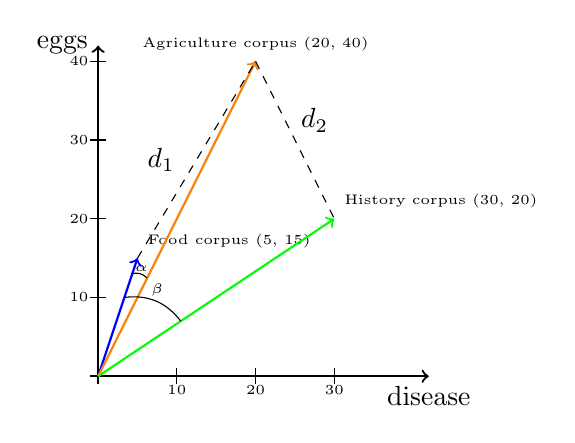
\begin{tikzpicture}
    \draw[->, thick] (-0.1, 0) -- (4.2, 0) node[below] {disease};
    \draw[->, thick] (0, -0.1) -- (0, 4.2) node[left] {eggs};
    % x-axis ticks
    \draw[-] (1, -0.1) -- (1, 0.1) node[below=1mm] {\tiny 10};
    \draw[-] (2, -0.1) -- (2, 0.1) node[below=1mm] {\tiny 20};
    \draw[-] (3, -0.1) -- (3, 0.1) node[below=1mm] {\tiny 30};
    % y-axis ticks
    \draw[-] (-0.1, 1) -- (0.1, 1) node[left=1mm] {\tiny 10};
    \draw[-] (-0.1, 2) -- (0.1, 2) node[left=1mm] {\tiny 20};
    \draw[-] (-0.1, 3) -- (0.1, 3) node[left=1mm] {\tiny 30};
    \draw[-] (-0.1, 4) -- (0.1, 4) node[left=1mm] {\tiny 40};
    \draw[->, thick, blue] (0, 0) -- (0.5, 1.5) node[above right] (fc) {\color{black} \tiny Food corpus (5, 15)};
    \draw[->, thick, orange] (0, 0) -- (2, 4) node[above] (ac) {\color{black} \tiny Agriculture corpus (20, 40)};
    \draw[->, thick, green] (0, 0) -- (3, 2) node[above right] (hc)     {\color{black} \tiny History corpus (30, 20)};
    \draw[dashed] (0.5, 1.5) -- (2,4);
    \node at (0.8, 2.75) {$d_1$};
    \draw[dashed] (2, 4) -- (3, 2);
    \node at (2.75, 3.25) {$d_2$};
    \draw (0.42, 1.3) edge[bend left] (0.62, 1.25);
    \node at (0.55, 1.37) {\tiny $\alpha$};
    \draw (0.325, 1) edge[bend left] (1.05, 0.7);
    \node at (0.75, 1.1) {\tiny $\beta$};
  \end{tikzpicture}
  \caption{Realize that $d_2 < d_1$ due to the fact that, as measured by Euclidean distance, they are more similar in \emph{magnitude}. In this case, the Agriculture and History corpora are much larger than the Food corpus; this causes their frequency counts along the dimensions of ``disease'' and ``eggs'' to be quite high, and their Euclidean distance is resultingly smaller than the distance between Food and Agriculture, which isn't intuitive. What about considering the cosine of the angle between the vectors as a measure of similarity? In this case $\alpha < \beta$, and it happens to be that cosine similarity is a better metric than Euclidean distance under this representation.}
\end{center}
\end{figure}

An alternative measure to Euclidean distance is Cosine similarity: i.e. the cosine of the inner angle between two vectors. If the angle is small, the cosine would be close to unit value, whereas if the angle is close to 90 degrees, the cosine approaches zero. Recall that a vector norm is defined as $\|v\| = \sqrt{\sum_{i=1}^n v_i^2}$ and an inner-product is defined by $\langle u, v \rangle = u \cdot v = \sum_{i=1}^n u_i \cdot v_i$. Then, we can define cosine similarity as
\[
  \texttt{Cosine-similarity}(u,v) = \frac{\langle u, v \rangle}{\|u\| \|v\|}
\]

If the input arguments (vectors) are perpendicular, the cosine of their inner angle is zero (since $\cos(90\degree) = 0$), whereas if they point in the same direction their cosine angle is unit valued (since $\cos(0\degree) = 1$, even if they have differing magnitudes).

\paragraph{Manipulating words in vector spaces} How can we manipulate vectors using vector arithmetic to make predictions? I.e. we will use manipulate vector representations to infer unknown relations among words. Suppose we have a vector space with countries and their capital cities. Perhaps we know that the capital of the U.S. is Washington D.C., but that we don't know the capital of Russia, and we further we'd like to use our knowledge of Washington D.C. with the U.S. to figure it out: it's as easy as applying linear algebra.

\begin{figure}
  \begin{center}
    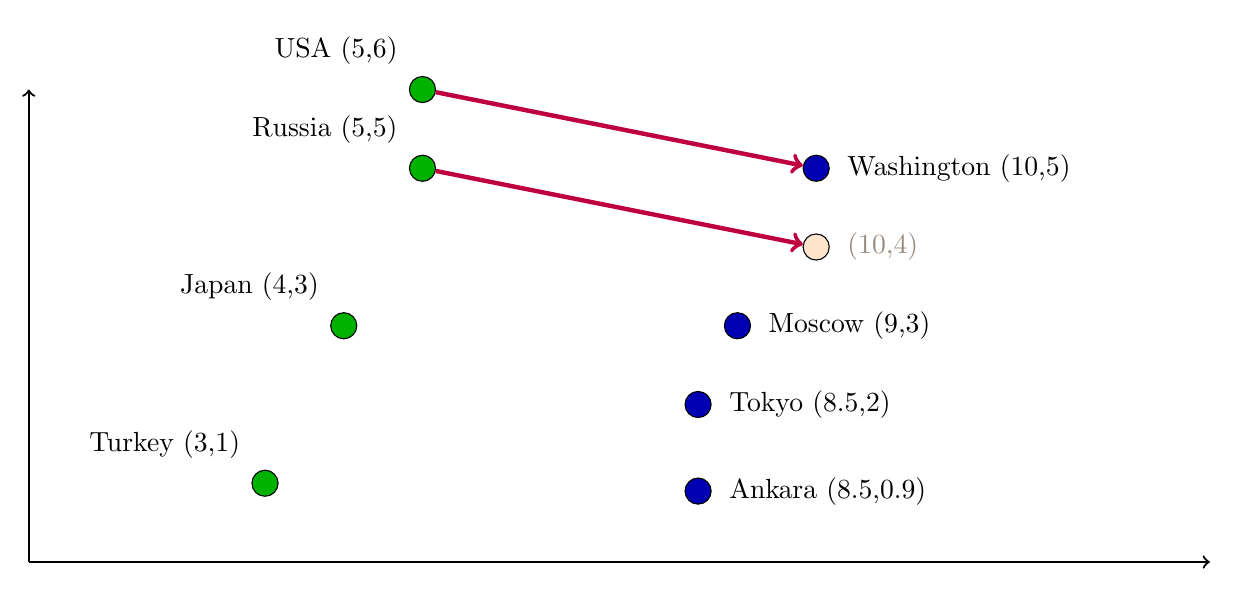
\begin{tikzpicture}
      \draw[->,thick] (0,0) -- (15, 0);
      \draw[->,thick] (0,0) -- (0, 6);
      \node[draw,circle,fill=green!70!black] (usa) at (5, 6) {};
      \node[draw,circle,fill=green!70!black] (russia) at (5, 5) {};
      \node[draw,circle,fill=green!70!black] (japan) at (4, 3) {};
      \node[draw,circle,fill=green!70!black] (turkey) at (3, 1) {};
      \node[draw,circle,fill=blue!70!black] (washington) at (10, 5) {};
      \node[draw,circle,fill=orange!20] (moscow_pred) at (10, 4) {};
      \node[draw,circle,fill=blue!70!black] (moscow) at (9, 3) {};
      \node[draw,circle,fill=blue!70!black] (tokyo) at (8.5, 2) {};
      \node[draw,circle,fill=blue!70!black] (ankara) at (8.5, 0.9) {};
      % Countries.
      \node[above left=1mm of usa] {USA (5,6)};
      \node[above left=1mm of russia] {Russia (5,5)};
      \node[above left=1mm of japan] {Japan (4,3)};
      \node[above left=1mm of turkey] {Turkey (3,1)};
      % Capitals.
      \node[right=1mm of washington] {Washington (10,5)};
      \node[right=1mm of moscow_pred] {\color{orange!20!black!50} (10,4)};
      \node[right=1mm of moscow] {Moscow (9,3)};
      \node[right=1mm of tokyo] {Tokyo (8.5,2)};
      \node[right=1mm of ankara] {Ankara (8.5,0.9)};
      % Relations
      \draw[->,ultra thick, purple] (usa) -- (washington);
      \draw[->,ultra thick, purple] (russia) -- (moscow_pred);
    \end{tikzpicture}
  \end{center}
  \caption{From \href{https://papers.nips.cc/paper/2013/file/9aa42b31882ec039965f3c4923ce901b-Paper.pdf}{Mikolov et. al. ``Distributed Representations of Words and Phrases and their Compositionality''}: in this representation, the vector between capitals Washington and USA is given by $[\texttt{Washington} - \texttt{USA}] = [5, -1]$. The easiest way to predict the capital of Russia is to simply take $\texttt{Russia} + [5, -1] = [10, 4]$. Because there are no cities with that representation, we'll search for the capital city that is most similar by comparing each vector with the Euclidean distances (or Cosine similarities). The catch is that we need a vector space where the representations capture the relative meaning of words.}
\end{figure}

\paragraph{Visualization and PCA} Often, we'll have vector representations in very high dimension, but we'll want to find a way to reduce the dimensions of the vectors to two dimensions so that we may plot it on a 2-D cartesian plane. What's the intuition? Principal Component Analysis is they key: it allows us to take a representation with $d > 2$ dimensions and project it down to a lower dimension, e.g. $d=2$, which we can then plot. If you perform PCA on your data, you might find that your word representation captures relationship between pairs of words that you expect to be related, in so far as these related words appear in clusters within the plot; you can confirm known relationships and also spot new ones using this technique.

\begin{figure}[h]
  \centering
  \begin{tikzpicture}[
    declare function={a(\x)=1;},
    declare     function={b(\x)=0;}
  ]
  \begin{axis}[
    domain=1:5,
    axis lines=middle,
    axis equal image,
    xtick=\empty,
    ytick=\empty,
    enlargelimits=true,
    clip mode=individual,
    clip=false
  ]
  \addplot [red, only marks, mark=x, samples=20, mark size=2]       {x*0.5*(a(x)+b(x)) + 0.5*rand*(a(x)-b(x))};
\end{axis}
\end{tikzpicture}
\caption{\footnotesize Raw data $(x_1, x_2)$ pairs.}
\end{figure}

\end{document}

